\section{Experiments}
\begin{table}[h]
\centering
\caption{
Performance comparison of different methods on \textit{\textbf{CSI 300}}.
We report both \textit{factor predictive power} and \textit{strategy-level performance} metrics, where \textbf{higher$\uparrow$} values  indicate better performance for all metrics (with the exception of MDD).
For each method category, the best result in each column is highlighted in \textbf{bold},
while the second-best result is \underline{underlined}.
Across all methods, the overall best-performing method is highlighted with a light \colorbox[RGB]{236,244,252}{blue background}.
}
\label{tab:csi300_results}
\setlength\tabcolsep{3.2pt}
\fontsize{8.1pt}{10.5pt}\selectfont
\begin{tabular}{llcccccccc}
\toprule[1.5pt]

\multicolumn{2}{c}{\multirow{2}{*}{\textbf{Methods}}} 
& \multicolumn{4}{c}{Factor Predictive Power}
& \multicolumn{4}{c}{Strategy Performance} \\
\cmidrule(lr){3-6} \cmidrule(lr){7-10}

\multicolumn{2}{c}{} 
& \textbf{IC} & \textbf{ICIR} & \textbf{Rank IC} & \textbf{Rank ICIR} 
& \textbf{IR (SHR*)} & \textbf{CR} & \textbf{ARR (\%)} & \textbf{MDD (\%)$\downarrow$} \\
\midrule[0.8pt]
\rowcolor[RGB]{230, 230, 230}\multicolumn{10}{c}{\textit{\textbf{Classical Factor Mining}}} \\
% ---------------- Machine Learning ----------------
\multirow{6}{*}{\textbf{Machine Learning}}
& Linear 
& 0.0155 
& 0.1174 
& 0.0368 
& 0.2834 
& -0.3078 
& -0.1407 
& -2.67 
& 18.97 \\


& XGBoost 
& 0.0175 
& 0.1336 
& 0.0420 
& 0.3417 
& -0.5280 
& -0.1488 
& -4.24 
& 28.50 \\

& CatBoost 
& 0.0162 
& 0.1203 
& 0.0405 
& 0.3289 
& -0.2807 
& -0.1077 
& -2.30 
& 21.35 \\

& LightGBM 
& \underline{0.0247} 
& \underline{0.2055} 
& \underline{0.0423} 
& \underline{0.3726} 
& 0.0092 
& 0.0032 
& 0.07 
& 21.80 \\


& MLP 
& \textbf{0.0321} 
& \textbf{0.2780} 
& \textbf{0.0438} 
& \textbf{0.4088} 
& \underline{0.1716} 
& \underline{0.0804} 
& \underline{1.46} 
& \underline{18.15} \\


& DoubleEnsemble 
& 0.0213 
& 0.1670 
& 0.0408 
& 0.3372 
& \textbf{0.2490} 
& \textbf{0.1233} 
& \textbf{1.85} 
& \textbf{15.00} \\

\midrule
% ---------------- Deep Learning ----------------
\multirow{4}{*}{\textbf{Deep Learning}}
& GRU 
& 0.0321 
& 0.2603 
& 0.0442 
& 0.3601 
& 0.5302 
& 0.2405 
& 3.61 
& 15.01 \\

& Transformer 
& \underline{0.0331} 
& \underline{0.2702} 
& \underline{0.0451} 
& \underline{0.3801} 
& 0.4502 
& 0.3773
& 5.21
& \underline{13.81} \\


& LSTM 
& \underline{0.0331} 
& 0.2502 
& \underline{0.0451} 
& 0.3503 
& \underline{0.6802} 
& \underline{0.4058} 
& \underline{6.01} 
& 14.81 \\

& TRA 
& \textbf{0.0421} 
& \textbf{0.3402} 
& \textbf{0.0511} 
& \textbf{0.4203} 
& \textbf{1.0502} 
& \textbf{0.8002} 
& \textbf{6.81} 
& \textbf{8.51} \\

\midrule
% ---------------- Factor Libraries ----------------
\multirow{3}{*}{\textbf{Factor Libraries}}
& Alpha158(20) 
& 0.0051 
& 0.0329 
& 0.0184 
& 0.1177 
& \underline{0.5044} 
& 0.2087 
& \textbf{4.63} 
& 22.19 \\

& Alpha158 
& \textbf{0.0131} 
& \textbf{0.0817} 
& \textbf{0.0334} 
& \textbf{0.2119} 
& 0.4099 
& \underline{0.2620} 
& 2.66 
& \textbf{10.15} \\

& Alpha360 
& \underline{0.0105} 
& \underline{0.0636} 
& \underline{0.0306} 
& \underline{0.1889} 
& \textbf{0.6009} 
& \textbf{0.3550} 
& \underline{4.09} 
& \underline{11.52} \\

\midrule[0.8pt]
\rowcolor[RGB]{230, 230, 230}\multicolumn{10}{c}{\textit{\textbf{LLM-based Agentic Factor Mining}}} \\
% \rowcolor[RGB]{230, 230, 230}{\multicolumn{10}{c}{LLM-based Agent}}
% ---------------- LLM R&D Agent ----------------
\multirow{5}{*}{\textbf{RD-Agent}}
& Qwen3-235B 
& 0.0352 
& 0.2850 
& 0.0485 
& 0.3950 
& 0.6502 
& 0.3591 
& 7.20 
& 20.05 \\

& Deepseek-V3.2 
& 0.0401 
& 0.3250 
& 0.0522 
& 0.4250 
& 0.8202 
& 0.4332 
& 7.81 
& 18.03 \\

& Gemini-3-pro-preview 
& 0.0481 
& 0.3900 
& 0.0583 
& 0.4750 
& 1.0202 
& 0.5499 
& 8.81 
& 16.02 \\

& Claude-4.5-sonnet 
& \underline{0.0527} 
& \underline{0.4250} 
& \underline{0.0623} 
& \underline{0.5050} 
& \underline{1.2202} 
& \underline{0.6488} 
& \underline{9.81} 
& \underline{15.12} \\

& GPT-5.2 
& \textbf{0.0531} 
& \textbf{0.4300} 
& \textbf{0.0633} 
& \textbf{0.5150} 
& \textbf{1.2502} 
& \textbf{0.6687} 
& \textbf{9.91} 
& \textbf{14.82} \\
\midrule
% ---------------- AlphaAgent ----------------
\multirow{5}{*}{\textbf{AlphaAgent}}
& Qwen3-235B 
& 0.0952 
& 0.6632 
& \underline{0.1019} 
& \underline{0.6471} 
& \underline{2.1053} 
& \underline{1.5945} 
& 15.10 
& \underline{9.47} \\

& Deepseek-V3.2 
& 0.0955 
& \underline{0.6637} 
& 0.0919 
& 0.6450 
& 1.9230 
& 1.4746 
& 14.51 
& 9.84 \\

& Gemini-3-pro-preview 
& 0.0804 
& 0.5366 
& 0.0784 
& 0.5290 
& 1.7821 
& 1.4729 
& 14.11 
& 9.58 \\

& Claude-4.5-sonnet 
& \textbf{0.1092} 
& \textbf{0.7718} 
& \textbf{0.1062} 
& \textbf{0.7596} 
& \textbf{2.2739} 
& \textbf{2.0246} 
& \textbf{16.48} 
& \textbf{8.14} \\

& GPT-5.2 
& \underline{0.0966} 
& 0.6344 
& 0.0942 
& 0.6237 
& 1.9328 
& 1.2056 
& \underline{15.54} 
& 12.89 \\

\midrule
% ---------------- QuantaAlpha ----------------
\multirow{5}{*}{\colorbox[RGB]{245, 235, 235}{\textbf{QuantaAlpha}}}
& Qwen3-235B 
& 0.1252 
& \underline{0.8672} 
& 0.1226 
& \underline{0.8577}
& 2.6114 
& 2.2859 
& 20.55 
& 8.99 \\

& Deepseek-V3.2 
& \underline{0.1338} 
& 0.8533 
& \underline{0.1300} 
& 0.8304
& \underline{2.8797} 
& 2.6007 
& \underline{23.77} 
& 9.14 \\





& Gemini-3-pro-preview 
& 0.1124 
& 0.7391 
& 0.1086 
& 0.7205 
& 2.5189 
& 2.1503 
& 20.32 
& 9.45 \\

& Claude-4.5-sonnet 
& 0.1111 
& 0.6374 
& 0.1077 
& 0.6211 
& 2.6459 
& \underline{3.2615} 
& 22.70 
& \colorbox[RGB]{236,244,252}{\textbf{6.96}} \\

& GPT-5.2 
& \colorbox[RGB]{236,244,252}{\textbf{0.1501}}
& \colorbox[RGB]{236,244,252}{\textbf{0.9110}}
& \colorbox[RGB]{236,244,252}{\textbf{0.1465}} 
& \colorbox[RGB]{236,244,252}{\textbf{0.8909}}
& \colorbox[RGB]{236,244,252}{\textbf{3.3251}}
& \colorbox[RGB]{236,244,252}{\textbf{3.4774}}
& \colorbox[RGB]{236,244,252}{\textbf{27.75}}
& \underline{7.98} \\


\bottomrule[1.5pt]
\end{tabular}
\end{table}









%  \begin{table}[tb]
%   \centering
%   \small
%   \caption{Ablation Study Results of QuantaAlpha's Constrain Gate Mechanisms}
%   \label{tab:constrain_gate_ablation}
%   \resizebox{\linewidth}{!}{
%     \begin{tabular}{l|ccc|cccccc}
%       \hline
%       \multirow{2}{*}{Model Variant} & \multicolumn{3}{c|}{Constrain Gate Mechanisms} & \multicolumn{6}{c}{Key Metrics} \\
%       \cline{2-10}
%       & Complexity Check & Redundancy Check & Consistency Check & IC & ICIR & ARR (\%) & IR (SHR*) & MDD (\%) & CR \\
%       \hline
%       QuantaAlpha (Full) & √ & √ & √ & \textbf{0.1494} & \textbf{0.9263} & \textbf{28.99} & \textbf{3.4828} & \textbf{-9.42} & \textbf{3.0763} \\
%       w/o Complexity Check & × & √ & √ & 0.1303 & 0.8173 & 23.51 & 2.7780 & -9.75 & 2.4113 \\
%       w/o Redundancy Check & √ & × & √ & 0.1252 & 0.8672 & 20.55 & 2.6114 & -11.99 & 1.7139 \\
%       w/o Consistency Check & √ & √ & × & 0.1223 & 0.8033 & 17.51 & 2.0776 & -10.69 & 1.6380 \\
%       \hline
%     \end{tabular}
%   }
%   \begin{tablenotes}
%     \small
%     \item  "w/o " denotes mechanism ablation; 
%   \end{tablenotes}
% \end{table}

\subsection{Experimental Setup}

\paragraph{Datasets and Metrics} We conduct experiments on the CSI 300 dataset, which covers 300 large-cap A-share stocks in the Chinese market. We adopt a chronological split with training (Jan. 1, 2016 to Dec. 31, 2020), validation (Jan. 1, 2021 to Dec. 31, 2021), and testing (Jan. 1, 2022 to Dec. 26, 2025). We evaluate performance from two complementary perspectives. Factor predictive power is measured by Information Coefficient (IC), IC Information Ratio (ICIR), Rank IC, and Rank ICIR. Strategy performance is measured by Annualized Return (ARR), Information Ratio (IR), Maximum Drawdown (MDD), and Calmar Ratio (CR). Further details are provided in Appendix~\ref{appendix:A.2}.

\paragraph{Baselines} We compare QuantaAlpha against four baseline categories: traditional machine learning models, deep learning time-series models, classical factor libraries, and LLM-based factor research agents, including RD-Agent and AlphaAgent. More details are provided in Appendix~\ref{appendix:A.5}.

\subsection{Main Results}
Table~\ref{tab:csi300_results} reports the main results on the CSI 300 market over a four-year evaluation period. QuantaAlpha outperforms all baselines on both factor predictive power and strategy-level performance. Using GPT-5.2, QuantaAlpha achieves the best IC at 0.1501, delivers an ARR of 27.75\%, and maintains a low MDD of 7.98\%. From a real-world perspective, this performance indicates that the mined factors can support production trading under standard risk controls, rather than being artifacts of backtest noise. Similarly, we observe consistent gains across different base models, suggesting that the improvements are robust rather than model-specific.

Compared with RD-Agent, QuantaAlpha and AlphaAgent both incorporate generation-stage regularization, and this is reflected in stronger predictive power and strategy performance. Under GPT-5.2, QuantaAlpha improves IC by 0.0970 and ARR by 17.84\% relative to RD-Agent while reducing MDD by 6.84\%, suggesting that constraining hypothesis-to-factor construction with explicit intermediate representations and verification effectively reduces semantic drift and improves implementation reliability. Beyond these constraints, QuantaAlpha further improves upon AlphaAgent by 0.0535 IC and 12.21\% ARR while reducing MDD by 4.91\%, highlighting the added value of trajectory-centric self-evolution: mutation broadens exploration via mechanism-level variations, while crossover reuses validated trajectory segments and repair strategies, jointly increasing the yield and stability of high-quality factors under non-stationary market dynamics.

\begin{figure}[t]
  \centering
  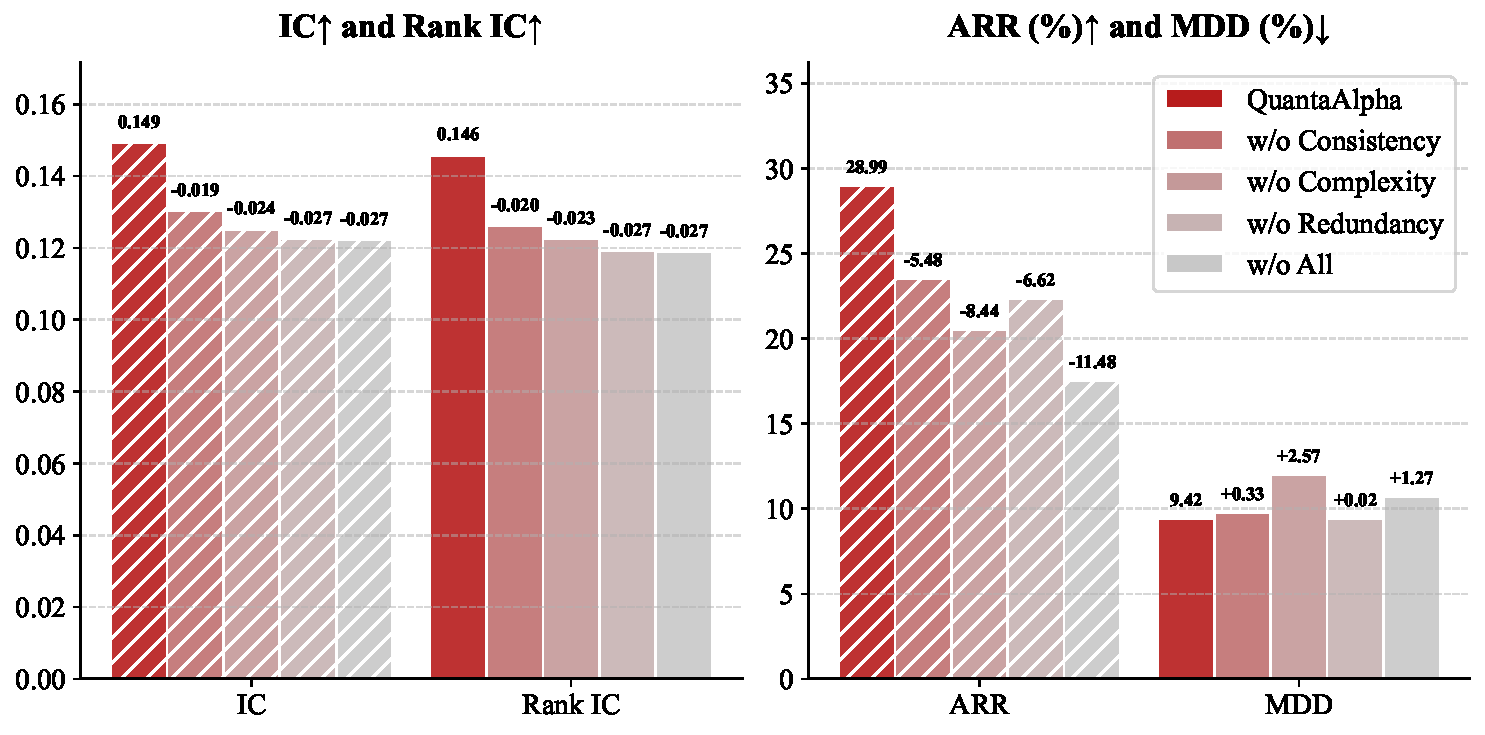
\includegraphics[width=0.8\columnwidth]{images/ablation.pdf}
  \caption{Ablation study of semantic consistency, complexity, and redundancy controls.}
  \label{fig:gate_ablation}
\end{figure}

\subsection{Ablation Study}
\paragraph{Ablation of Evolutionary Mining Components} We conduct an ablation study to quantify the contribution of three components in evolutionary alpha mining: diversified planning initialization, trajectory mutation, and trajectory crossover. The results are summarized in Table~\ref{tab:ablation_study_two_column}. Removing \emph{planning} yields only marginal changes in IC and Rank IC, but substantially degrades strategy-level outcomes, with ARR decreasing by 7.78\% and MDD increasing by 2.73\%. This indicates that diversified initialization primarily improves the search frontier by providing broader and less correlated starting hypotheses, which stabilizes subsequent evolution. In contrast, removing \emph{mutation} causes the largest drop in predictive power, decreasing IC by 0.0292 and Rank IC by 0.0284, and also leads to the largest reduction in ARR by 9.81\%. This highlights mutation as the primary driver of effective exploration and trajectory repair, enabling the system to escape suboptimal regions and correct failure modes discovered during mining. Meanwhile, removing \emph{crossover} leads to a smaller but consistent degradation. This supports the role of crossover in exploiting and inheriting complementary high-performing trajectory segments, improving efficiency and stability by recombining validated patterns from successful trajectories.
\begin{table}[h]
  \centering
  \normalsize % 核心跨档放大：从\scriptsize直接升级为\normalsize（文档默认正文字体，单栏表格大幅放大的最优选择）
  \caption{Ablation study of evolutionary mining components.}
  \label{tab:ablation_study_two_column}
  \setlength{\tabcolsep}{10pt} % 大幅舒展列间距（适配\normalsize字体，单栏下不超界且不冗余）
  \begin{tabular}{lcccc}
    \toprule
   \multirow{2}{*}{Method} & \multicolumn{4}{c}{Key Metrics} \\
    \cmidrule(lr){2-5}
     &  \multicolumn{1}{l}{\,\,\,\textbf{IC}} &  \multicolumn{1}{l}{\textbf{Rank IC}} &  \multicolumn{1}{l}{\textbf{ARR}} (\%) & \textbf{MDD} (\%) $\downarrow$\\
    \midrule

     \textbf{QuantaAlpha}
& \multicolumn{1}{l}{\textbf{0.1493}}
& \multicolumn{1}{l}{\textbf{0.1458}}
& \multicolumn{1}{l}{\textbf{28.99}}
& \multicolumn{1}{l}{\,\,\,\,\textbf{9.42}} \\

     \phantom{Q} -  \emph{w/o} \textbf{Planning}
      & 0.1488\textsuperscript{\textcolor[RGB]{230,180,180}{\tiny -0.0005}}
      & 0.1452\textsuperscript{\textcolor[RGB]{230,180,180}{\tiny -0.0006}}
      & 21.21\textsuperscript{\textcolor[RGB]{180,20,20}{\tiny -7.78}}
      & 12.15\textsuperscript{\textcolor[RGB]{200,50,50}{\tiny +2.73}} \\

     \phantom{Q} -  \emph{w/o} \textbf{Mutation}
      & 0.1201\textsuperscript{\textcolor[RGB]{180,60,60}{\tiny -0.0292}}
      & 0.1174\textsuperscript{\textcolor[RGB]{180,60,60}{\tiny -0.0284}}
      & 19.18\textsuperscript{\textcolor[RGB]{160,20,20}{\tiny -9.81}}
      & 9.85\textsuperscript{\textcolor[RGB]{220,160,160}{\tiny +0.43}} \\

      \phantom{Q} -  \emph{w/o} \textbf{Crossover}
      & 0.1423\textsuperscript{\textcolor[RGB]{220,150,150}{\tiny -0.0070}}
      & 0.1381\textsuperscript{\textcolor[RGB]{220,150,150}{\tiny -0.0077}}
      & 26.17\textsuperscript{\textcolor[RGB]{200,50,50}{\tiny -2.82}}
      & 10.63\textsuperscript{\textcolor[RGB]{220,100,100}{\tiny +1.21}} \\

    \bottomrule
  \end{tabular}
\end{table}


\paragraph{Ablation of Consistency, Complexity, and Redundancy Controls} We ablate three controls during factor generation that gate rewriting, including semantic consistency verification, complexity regularization, and redundancy filtering. As shown in Figure~\ref{fig:gate_ablation}, disabling any single control consistently degrades performance, confirming that each contributes non-trivially to robust factor generation. The \emph{consistency} control prevents semantic drift between the hypothesis, symbolic specification, and implementation. The \emph{complexity} control improves robustness by discouraging overly complex expressions that generalize poorly, and its removal leads to the most pronounced degradation at the strategy level, with the annualized excess return dropping by 8.44\% and the maximum drawdown increasing by 2.57\%. The \emph{redundancy} control preserves exploration by filtering near-duplicate structures and mitigating factor crowding. Disabling all three yields the largest degradation, indicating that these controls are complementary and jointly needed for reliable generation.

\subsection{More Analysis}

\paragraph{Factor Generalizability} To evaluate factor robustness under significant market distribution shifts, we conduct a zero-shot transfer experiment where the factors mined and selected on CSI 300 are directly deployed on CSI 500 and the S\&P 500 without any re-optimization or market-specific adaptation. As shown in Figure~\ref{fig:cumulative_returns}, QuantaAlpha demonstrates substantially stronger out-of-distribution generalization than all baselines. A clear divergence emerges around December 2023, when competing methods begin to stagnate under shifts in market microstructure and volatility regimes, whereas QuantaAlpha sustains a stable upward trajectory. By the end of the evaluation period, it reaches a cumulative excess return of roughly \textbf{160\%} on CSI 500 and over \textbf{137\%} on the S\&P 500. These results indicate that the discovered factors transfer beyond the source market and retain effectiveness under distribution shifts, rather than relying on market-specific historical patterns.

\paragraph{Alpha Decay} Figure~\ref{fig:annual_ic_rankic} reports annual IC and Rank IC on the CSI~300 universe from 2021 to 2025. A pronounced performance collapse is observed for the baselines in 2023, coinciding with a major regime shift in the A-share market. The pre-2023 period is dominated by large-cap ``core assets'', where institutional trading supports relatively stable trends and makes classical momentum or mean-reversion signals effective. In 2023, the market rotates toward small-cap and thematic stocks, together with higher intraday noise, more frequent overnight gaps, and weaker trend persistence. Baseline methods, whose factor libraries implicitly assume smooth trends and regular reversal patterns, fail to transfer to this out-of-distribution environment. QuantaAlpha, by comparison, maintains strong IC and Rank IC through the regime transition. It discovers more structural factors, such as \textit{Mean-Reverting Range Deviation} and \textit{Overnight Gap Structure}, that reflect persistent microstructure effects including volatility clustering and overnight information incorporation. These signals are less sensitive to capitalization style, enabling better temporal generalization. 
\begin{figure}[h]
\centering
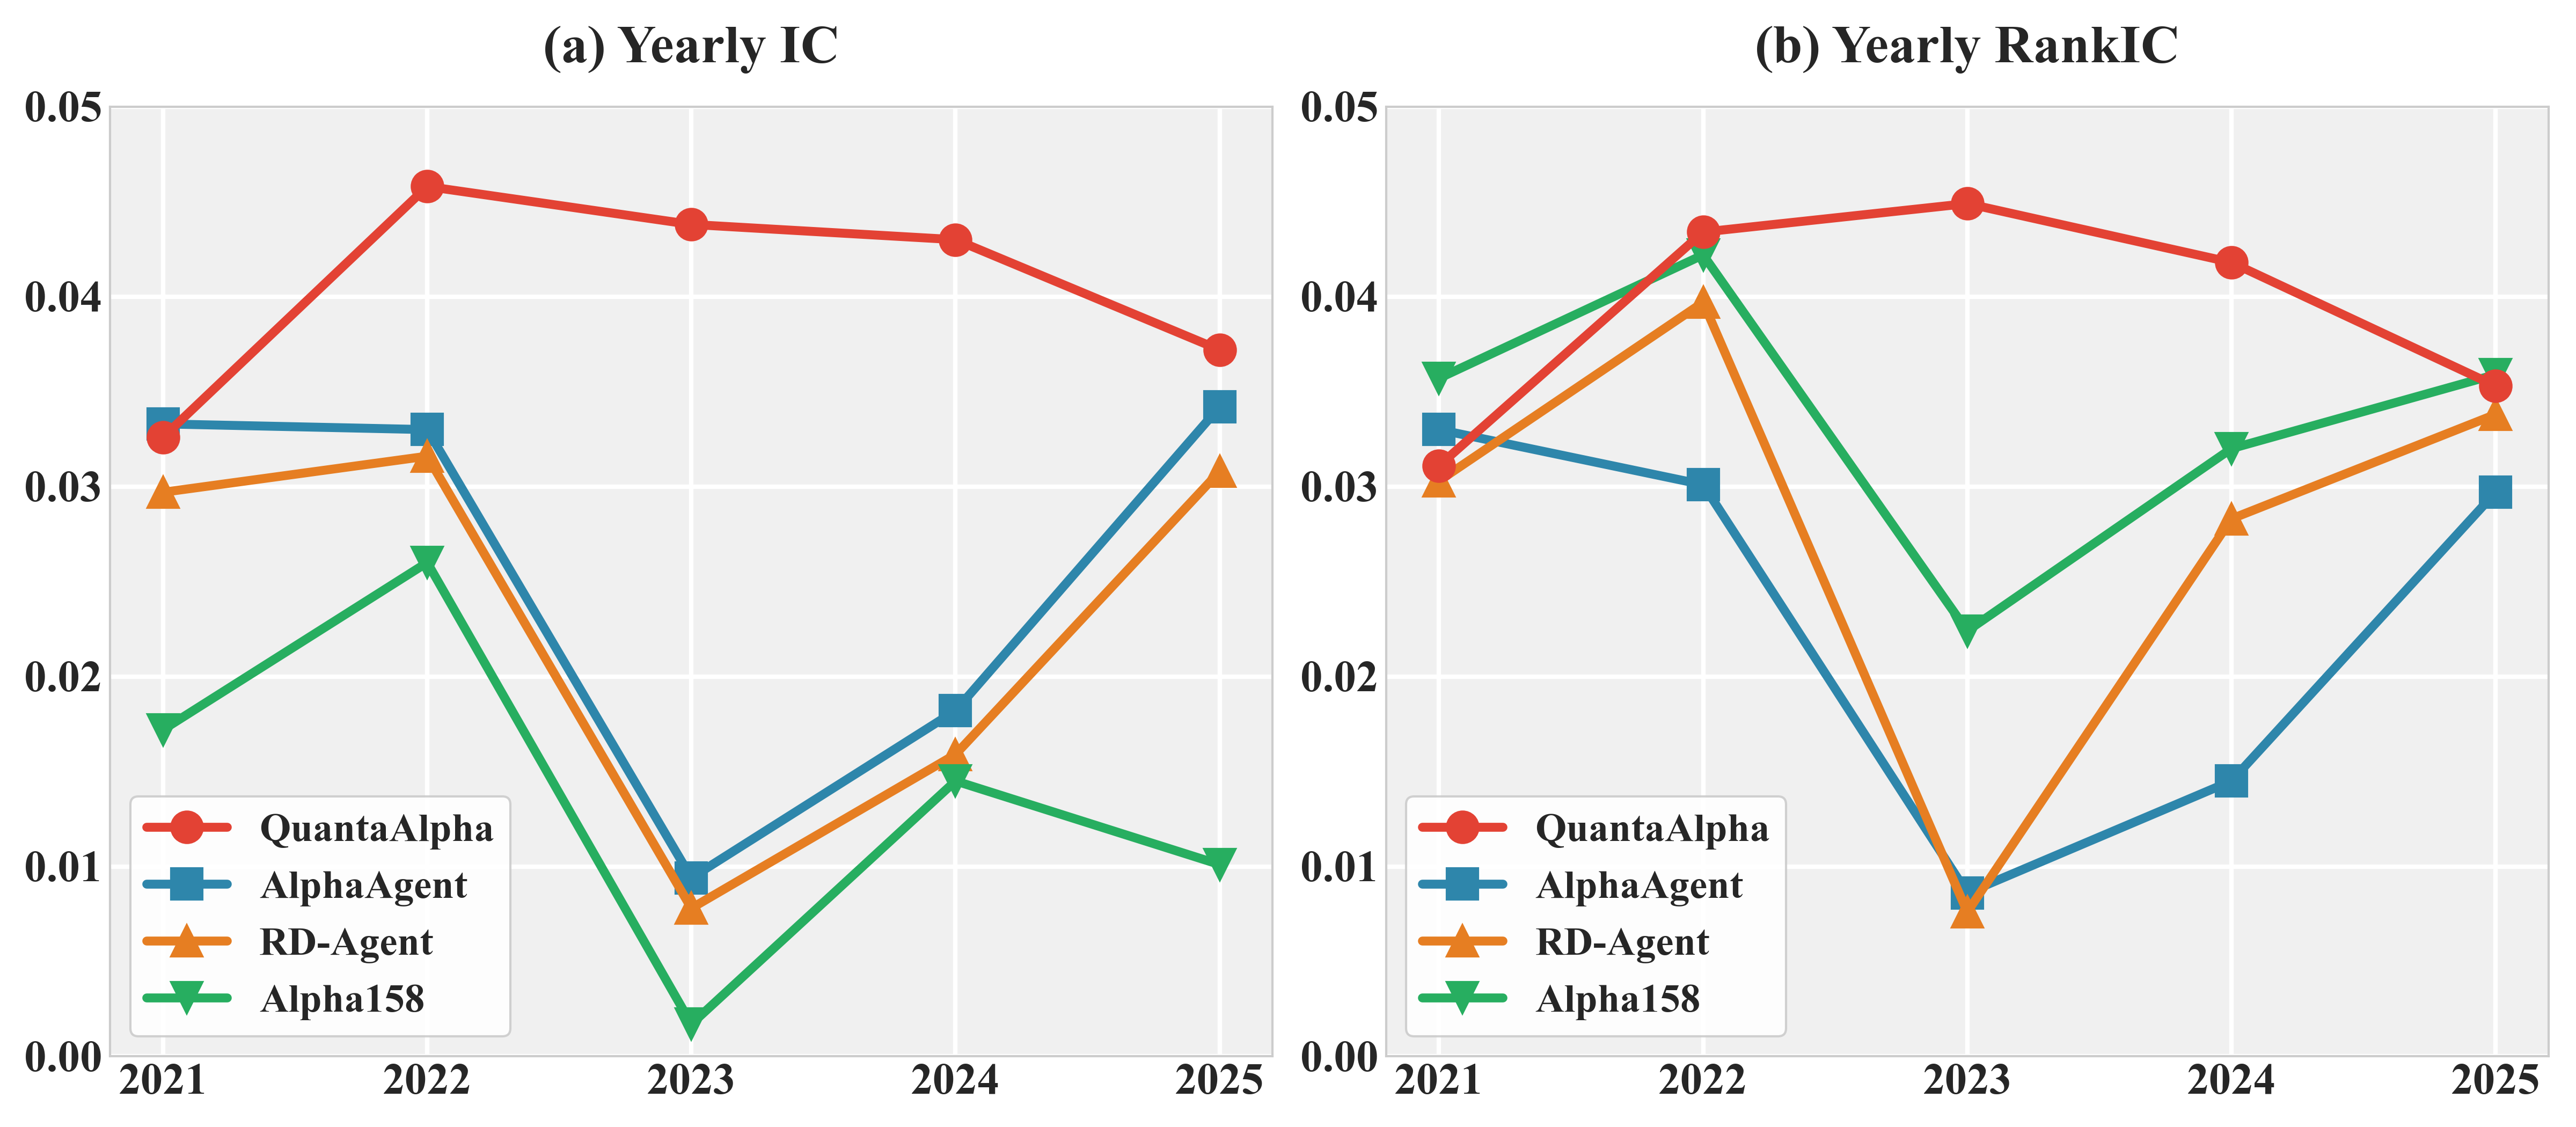
\includegraphics[width=0.8\columnwidth]{images/figure4.png} 
\caption{Annual IC and Rank IC comparison on the CSI 300.}
\label{fig:annual_ic_rankic}
\end{figure}

Table~\ref{tab:qa_aa_2023_representative} provides a factor-level diagnosis of the alpha decay observed in 2023, grounding the analysis jointly in \emph{market style changes}, \emph{factor semantics}, and \emph{empirical factor statistics}.  
Rather than enumerating factor formulas, we focus on which information channels remain predictive under the 2022--2023 regime transition and why.

\paragraph{Market Style Transition and Its Implications}

The CSI~300 market undergoes a pronounced style transition in 2023 relative to the training period (2016--2020).  
The earlier regime is dominated by large-cap core assets, with high institutional participation, smooth intraday dynamics, and persistent short-horizon trends. Under such conditions, classical momentum, mean-reversion, and exhaustion-based factors are effective.In 2023, leadership rotates toward small-cap and thematic stocks. This shift is accompanied by increased intraday noise, frequent overnight gaps driven by call auctions, and rapid cross-style liquidity re-allocation. These changes weaken trend persistence and amplify path-dependent noise, directly challenging factor constructions that rely on stable intraday structure or fast mean reversion.

\paragraph{Factor Semantics Aligned with Market Microstructure}

The empirical contrast between QuantaAlpha (QA) and AlphaAgent (AA) in 2023 reflects differences in the \emph{semantic composition} of their factor libraries.

\textbf{(i). Overnight and auction information.}
Gap-based factors aggregate information released during non-trading hours and price discovery in the opening auction.  
As shown in Table~\ref{tab:qa_aa_2023_representative}, multiple QA factors from this channel occupy the right tail of the 2023 Rank IC distribution, while maintaining near-complete coverage (Table~\ref{tab:qa_aa_2023_summary}). This indicates that overnight information becomes a dominant and stable signal when intraday predictability deteriorates.

\begin{table*}[!t] \centering \caption{Representative factors and their performance metrics on the CSI 300 index in 2023.} \label{tab:qa_aa_2023_representative} \scriptsize \setlength{\tabcolsep}{3pt} \renewcommand{\arraystretch}{1.06} \begin{tabular}{p{5.8cm}ccp{8.2cm}} \toprule \textbf{Factor (representative)} & \textbf{Rank IC} & \textbf{IC} & \textbf{Interpretation (short)} \\ \midrule \multicolumn{4}{c}{\textit{QA --- strong performers (overnight/auction, trend-quality, and liquidity re-rating)}} \\ \midrule \texttt{GapZ10\_Overnight\_vs\_TR} & 0.0793 & 0.0335 & Normalized overnight gap magnitude relative to recent true range; captures auction-driven shocks and subsequent adjustment. \\ \texttt{Gap\_IntradayAcceptanceScore\_20D} & 0.0744 & 0.0330 & `Acceptance vs.\ rejection'' of an overnight gap using intraday direction, scaled by recent volatility. \\ \texttt{Gap\_IntradayAcceptance\_VolWeighted\_20D} & 0.0606 & 0.0314 & Gap acceptance score weighted by abnormal volume; emphasizes information-rich openings with high participation. \\ \texttt{CleanTrend\_Continuation\_Score\_RS10\_WVMA5} & 0.0590 & 0.0267 & Trend continuation conditioned on high trend quality (low residual noise) and muted intraday/volume pressure. \\ \texttt{OrderlyTrend\_x\_Absorption\_10D\_5D\_20D} & 0.0465 & 0.0271 & `Orderly'' short-horizon trend cross-validated by liquidity absorption (high dollar volume with low price impact). \\ \midrule \multicolumn{4}{c}{\textit{QA --- weak performers (overly rigid gates or noisy-path proxies under rotation)}} \\ \midrule \texttt{KineticLength\_AbsRetSum\_Z\_10D} & -0.0720 & -0.0246 & Path-length proxy (choppiness): can behave like a noise detector, but may invert under fast style rotation. \\ \texttt{Drawdown\_Gated\_NegCorr\_60D\_20D\_thr20pct} & -0.0282 & -0.0095 & Hard regime gate based on deep drawdown; brittle when drawdowns cluster and cross-sectional regimes shift quickly. \\ \texttt{HighClose\_Shock\_With\_VolSync\_60\_20} & -0.0274 & -0.0090 & `Shock-day'' breakout quality (close-in-range, range shock, return--volume sync); sensitive to regime-dependent follow-through. \\ \midrule \multicolumn{4}{c}{\textit{AA --- strong performers (exhaustion/climax-style reversals)}} \\ \midrule \texttt{Exhaustion\_Intensity\_Index\_10D} & 0.0323 & 0.0159 & Price displacement over 60D interacted with volume intensity ratio; targets potential exhaustion and reversal. \\ \texttt{Climax\_Exhaustion\_Intensity} & 0.0242 & 0.0160 & Variant using short-horizon volume climax vs.\ long-horizon baseline; aims to identify capitulation-like turns. \\ \texttt{Exhaustion\_Volume\_Instability\_Index} & 0.0121 & 0.0117 & Trend deviation combined with volume instability; highlights fragile price levels supported by unstable liquidity. \\ \midrule \multicolumn{4}{c}{\textit{AA --- weak performers (bottom-fishing under non-stationary liquidity)}} \\ \midrule \texttt{Relative\_Volume\_Calm\_Reversal} & -0.0279 & -0.0188 & `Quiet-volume'' regimes multiplied by momentum divergence; may fail when liquidity conditions change abruptly. \\ \texttt{Volume\_Stability\_Momentum\_Divergence\_40D} & -0.0247 & -0.0155 & Robust volume-stability proxy (MAD) times momentum spread; sensitive to turnover regime changes. \\ \texttt{LVR\_Bottom\_Fishing\_20D} & -0.0190 & -0.0144 & `Bottom-fishing'' reversal with intraday rejection and volume surge; vulnerable when reversals are short-lived and crowded. \\ \bottomrule \end{tabular} \end{table*}

\begin{table}[!htbp] \centering \caption{Summary statistics of annual factor predictability on the CSI 300 index in 2023.} \label{tab:qa_aa_2023_summary} \small \setlength{\tabcolsep}{5pt} \begin{tabular}{lcc} \toprule \textbf{Metric} & \textbf{QA} & \textbf{AA} \\ \midrule Coverage ratio (valid metrics) & 0.98 & 0.80 \\ Share with Rank IC $>0$ & 0.626 & 0.594 \\ Mean Rank IC & 0.0057 & 0.0012 \\ Max Rank IC & 0.0793 & 0.0323 \\ Min Rank IC & -0.0720 & -0.0279 \\ Share with Rank IC $>0.03$ & 0.102 & 0.0156 \\ Share with Rank IC $>0.05$ & 0.0272 & 0.0000 \\ \midrule Mean IC & 0.0044 & 0.0015 \\ \bottomrule \end{tabular} \end{table}

\textbf{(ii). Volatility structure and range-based signals.}
Range deviation factors conditioned on volatility clustering capture abnormal variability rather than directional trends.  
In 2023, these signals remain predictive despite elevated noise, consistent with the persistence of volatility clustering across market styles. Their contribution is reflected in the heavier positive Rank IC tail of QA relative to AA.

\textbf{(iii). Trend quality and liquidity re-rating.}
QA emphasizes trend continuation only when supported by low residual volatility and improving liquidity (e.g., rising dollar volume with limited price impact).  
This conditioning filters out noise-driven pseudo-trends prevalent in small-cap rotation, explaining why QA retains a higher fraction of strong-performing factors, whereas raw momentum proxies degrade.

\paragraph{Factor Statistics as Supporting Evidence} The factor-level statistics in 2023 provide quantitative support for the semantic interpretation above.  
QA achieves substantially higher coverage and a heavier right tail of Rank IC, including a non-trivial share of factors exceeding moderate predictability thresholds, whereas AA exhibits compressed tails and fewer robust signals.  
These differences are consistent with the dominance of overnight, volatility-structure, and trend-quality channels under the 2023 market style.

A key distinction is that QA explicitly encourages semantic diversity through its factor mutation mechanism.  
By generating and recombining heterogeneous primitives across multiple information channels, QA avoids concentration on a single market hypothesis.  
This diversity increases the probability that a subset of factors remains aligned with the prevailing market microstructure after a style transition, thereby mitigating regime-specific alpha decay.
Overall, the 2023 diagnosis indicates that alpha robustness under distribution shift is driven by alignment between market style and factor semantics, supported by sufficient diversity across information channels.  
QA’s ability to maintain performance arises not from fitting a specific regime, but from sustaining a broad and adaptive factor population whose predictive subsets persist across market style transitions.



\paragraph{Evolutionary Alpha Mining Efficiency} We analyze the iterative dynamics of factor mining by tracking the IC distribution across generation rounds.
As visualized in Figure~\ref{fig:ic_evolution}, QuantaAlpha consistently maintains the highest IC across all five iterations, indicating that its evolutionary updates improve factor quality more effectively than both AlphaAgent and RD-Agent. Notably, QuantaAlpha exhibits a rapid gain in the early rounds and then remains stable at a high level, suggesting strong sample efficiency in converting early exploration into consistently predictive factors. In addition to the higher mean, QuantaAlpha shows a moderate but persistent spread of IC across rounds, reflecting sustained diversity in the explored factor candidates rather than premature collapse to a narrow region. By comparison, RD-Agent remains lower with relatively homogeneous IC profiles, consistent with weaker exploration and a higher risk of generating crowded signals. AlphaAgent improves over RD-Agent but remains consistently below QuantaAlpha, suggesting that our trajectory-level evolution more efficiently accumulates and reuses successful generation patterns across iterations.

\begin{figure}[h]
\centering
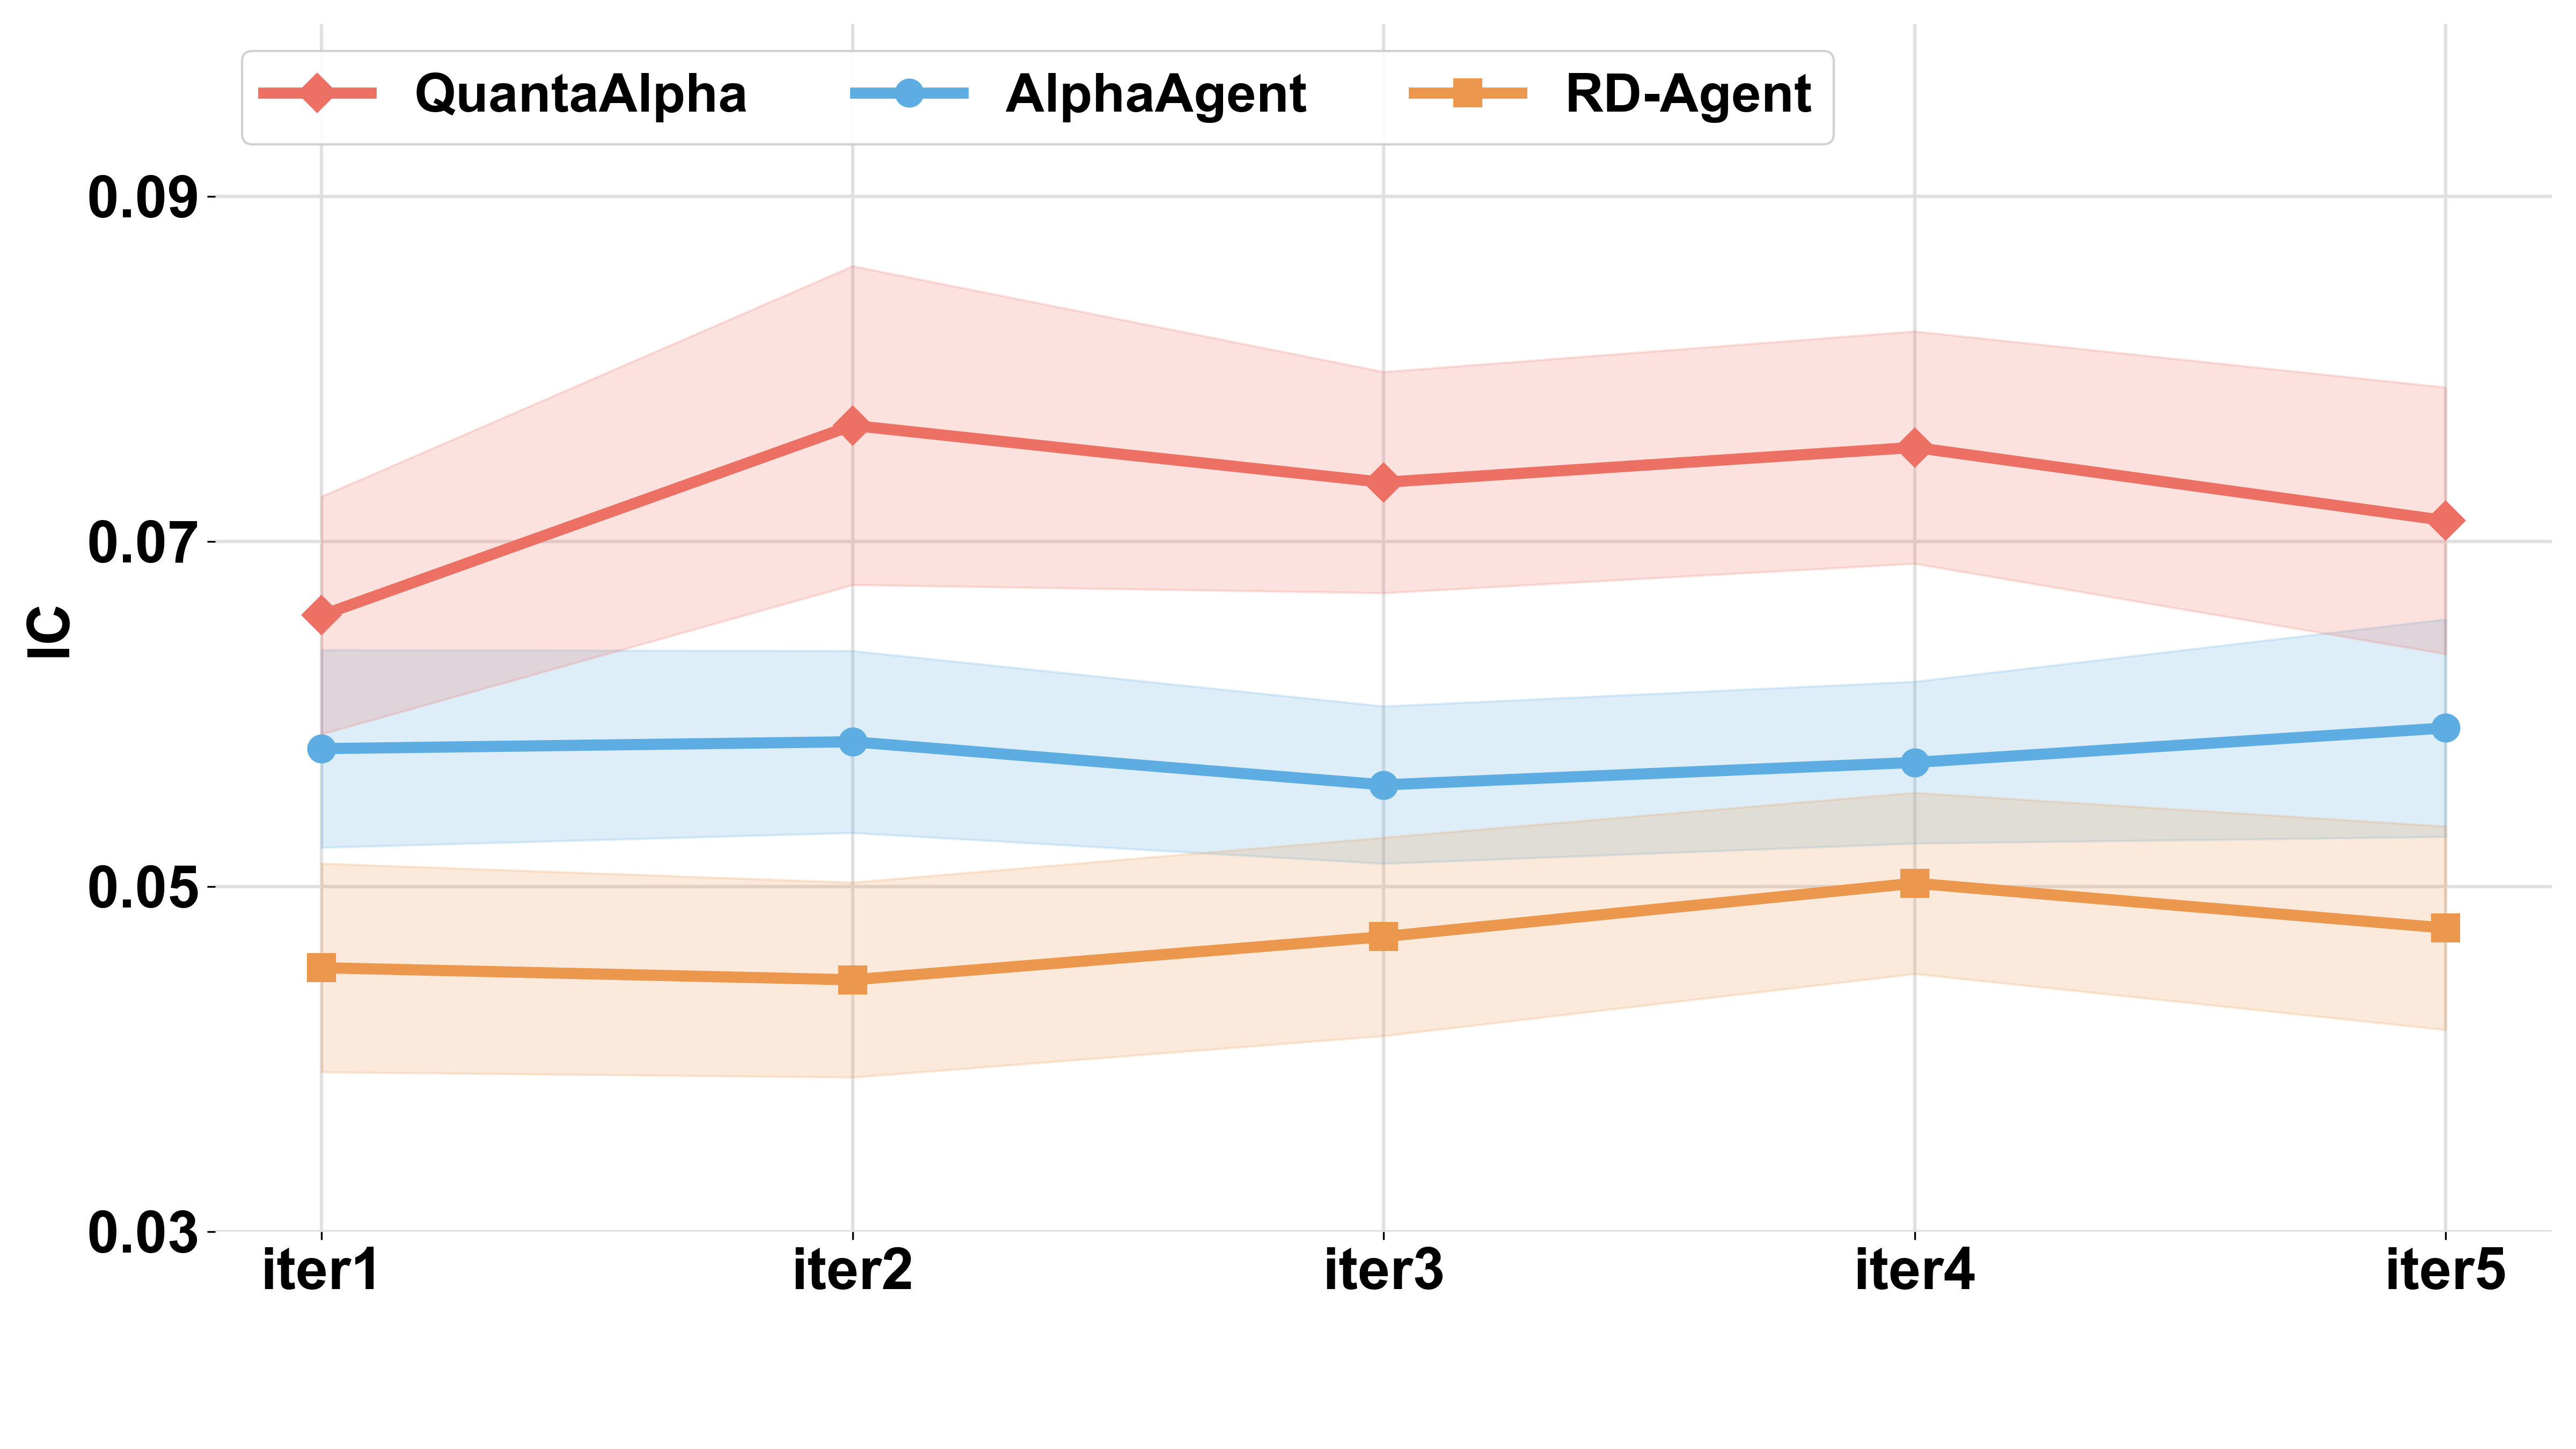
\includegraphics[width=0.6\columnwidth]{images/figu.png}
\caption{The evolution of IC over the first five iterations.}
\label{fig:ic_evolution}
\end{figure}

\subsection{Case Study}
\paragraph{Case Study Setup} To make the evolution process concrete, we present a representative case study and trace how QuantaAlpha updates hypotheses and factors over five iterations. We run QuantaAlpha for a total of 15 iterations on CSI300, using Deepseek-V3.2 as the backbone LLM for all agents. To improve mining throughput, we set the factor-complexity constraints to symbol length $\leq 200$ and base features $\leq 4$. Each iteration consists of two phases: a \textit{Mutation} phase followed by a \textit{Crossover} phase.At the end of each iteration, we maintain a global high-quality factor pool using all factors generated up to that iteration. The maintenance rule is greedy and RankIC-driven: we sort all candidate factors by RankIC (descending) and add them into the pool in order, subject to a redundancy constraint. A factor is admitted only if its absolute correlation with every factor already in the pool is below 0.7. The pool size is capped at 50\% of the total number of mined factors up to the current iteration. 

\begin{figure}[!t]
\centering
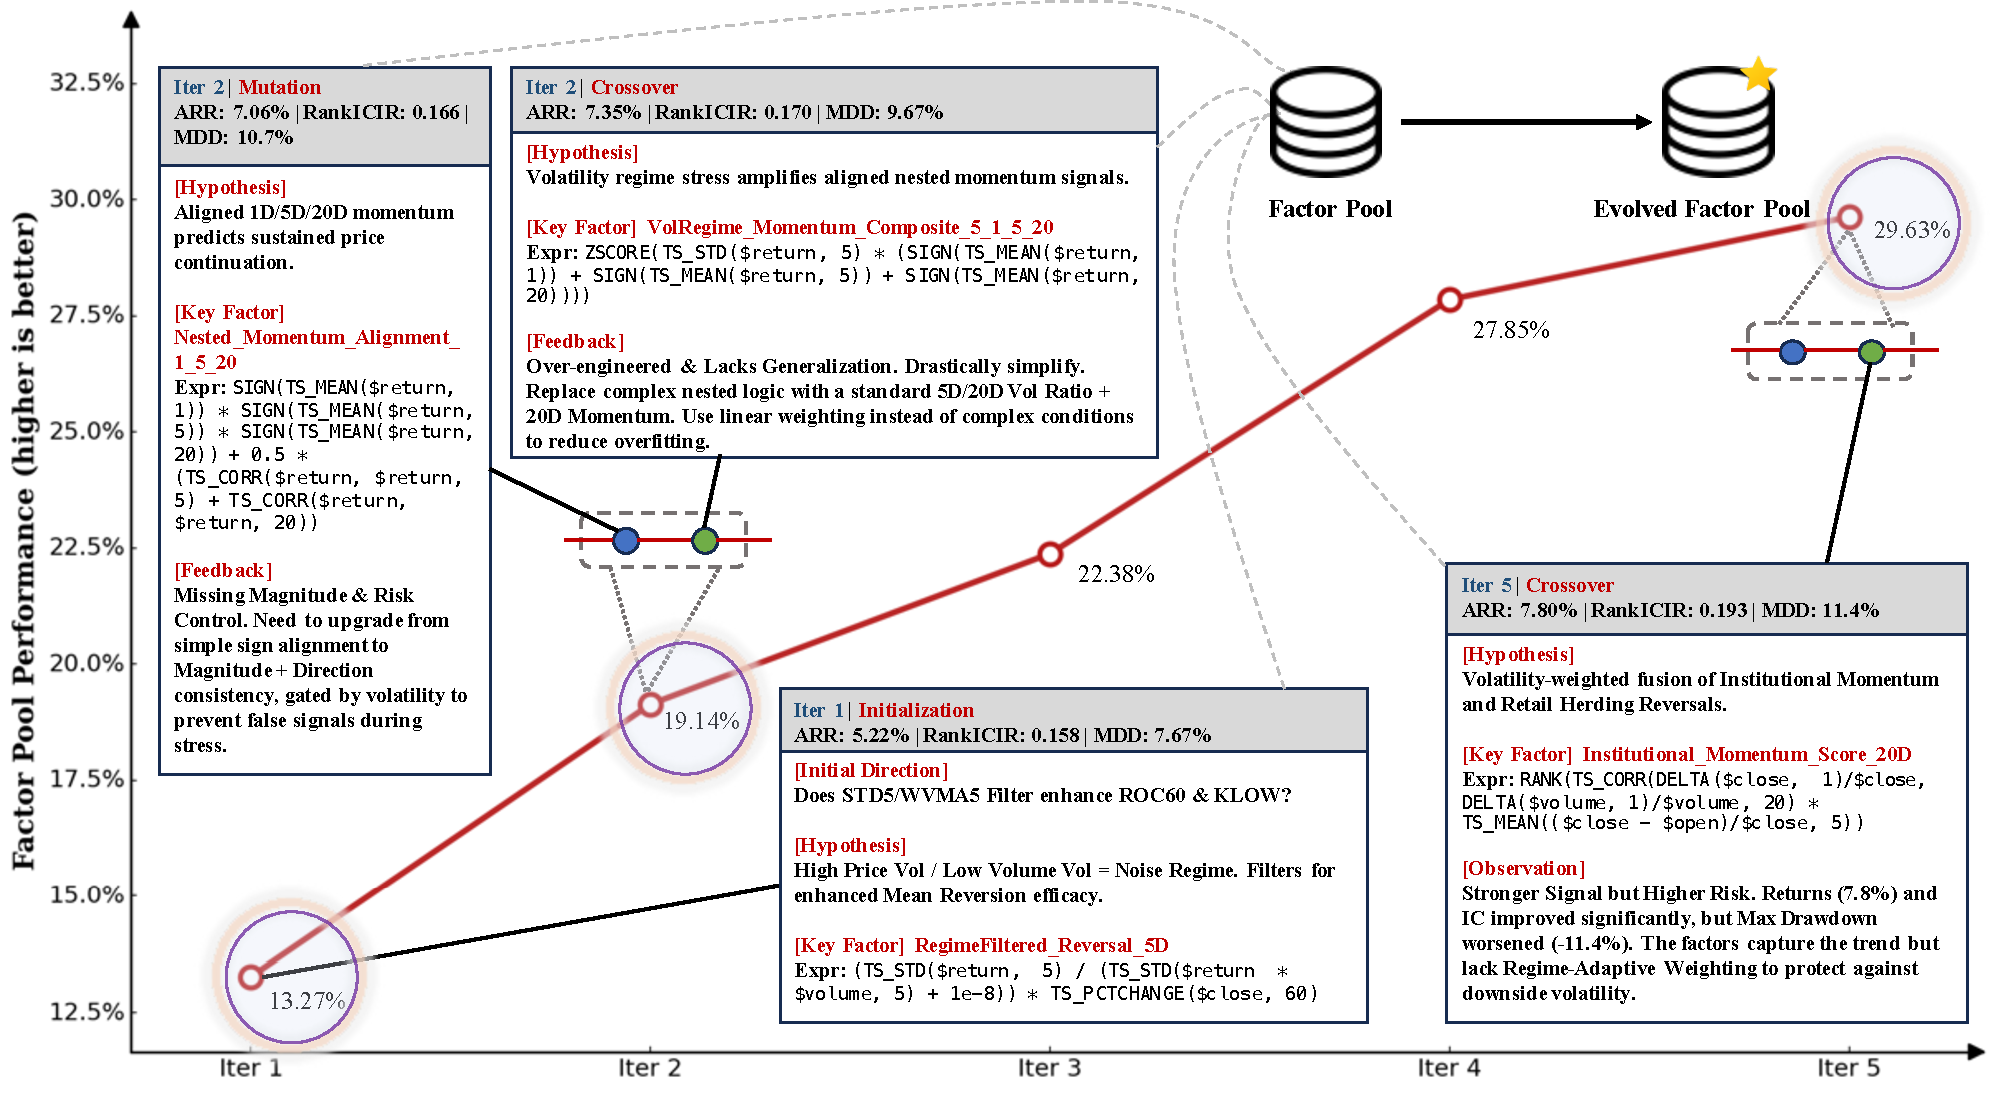
\includegraphics[width=1\textwidth]{images/case_study.pdf}
\caption{A case study of iterative hypothesis and factor updates in QuantaAlpha.}
\label{fig:case_study}
\end{figure}


\paragraph{Factor Example} Figure~\ref{fig:case_study} illustrates how QuantaAlpha refines hypotheses and factor expressions across iterations via the \emph{mutation} and \emph{crossover} phases. The highlighted factors in the figure are therefore representative nodes on different traces across iterations. The first iteration yields interpretable short-term reversal factors. The second broadens the mechanism via volatility-weighted momentum, but increased structural complexity coincides with weaker generalization. Subsequent iterations simplify the expression into a linear additive form, improving drawdown and stabilizing performance. The fifth iteration adds participant-differentiated behavioral signals, incorporating complementary information and further improving predictability. Throughout the evolution, QuantaAlpha maintains a cumulative factor pool. Its predictive performance does not saturate within the first five iterations and only begins to decay after roughly 15 iterations, indicating that the evolution sustains effective improvement over a substantial horizon before diminishing returns emerge.  

\paragraph{Iteration Convergence} Figure~\ref{fig:Iteration_analysis_appendix} illustrates the predictive performance of the factor pool from the fifth iteration onwards. We observe that the predictive performance does not increase linearly with the number of iterations. The strategy's return capacity and risk control ability are gradually optimized, reaching a balanced high level between return and maximum drawdown around the 11th to 12th iterations. Subsequent additional iterations fail to bring significant performance improvement; instead, they may introduce redundant information through newly generated factors, leading to reduced strategy robustness and deteriorated drawdown performance. Overall, the 11th to 12th iterations (approximately 350 factors in total) represent the optimal trade-off point between return level and risk control effect under this experimental setup.


\begingroup
\makeatletter
% If LaTeX decides to put this figure on a float-only page, remove vertical centering.
\setlength{\@fptop}{0pt}
\setlength{\@fpbot}{0pt}
\makeatother
\begin{figure}[!t]
\centering
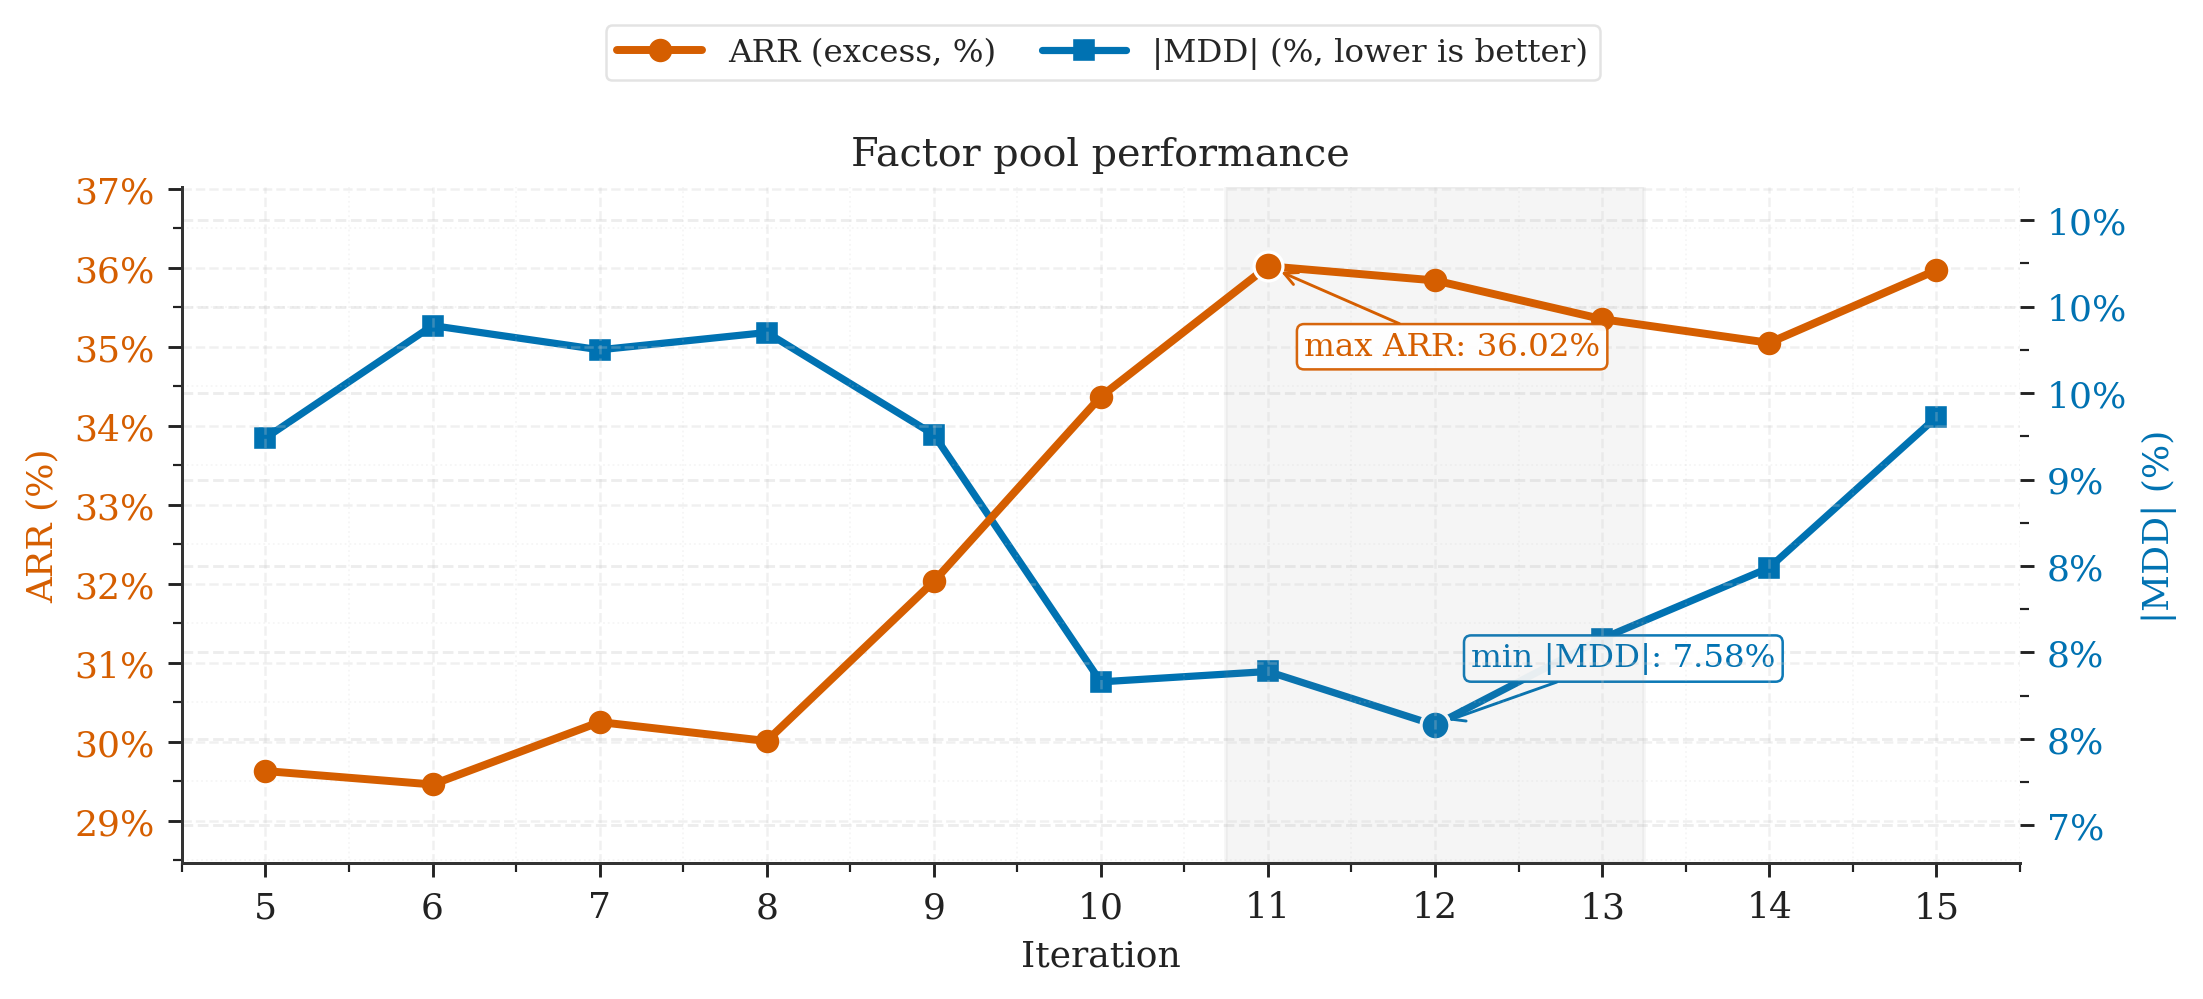
\includegraphics[width=0.95\textwidth]{images/iteration.png}
\caption{Factor Pool Performance by Iteration.}
\label{fig:Iteration_analysis_appendix}
\end{figure}
\endgroup
